\documentclass{beamer}

% ---------- Theme & formatting ----------
\usetheme{Madrid}
\usecolortheme{default}
\setbeamertemplate{navigation symbols}{}
\setbeamertemplate{caption}[numbered]
\setbeamertemplate{footline}[frame number]
\beamertemplatenavigationsymbolsempty

% ---------- Packages ----------
\usepackage{amsmath, amsfonts, amssymb}
\usepackage{booktabs, multirow, array}
\usepackage{hyperref}
\usepackage{siunitx}
\usepackage{tikz}
\usepackage{pgfplots}
\pgfplotsset{compat=1.18}
\usetikzlibrary{arrows.meta, positioning, calc, shapes.geometric, shapes.misc, fit}

% ---------- Title ----------
\title[RMSTSS]{RMSTSS: A Comprehensive Suite for Power \& Sample Size Using Restricted Mean Survival Time (RMST)}
\author[Arnab Aich, Yuan Zhang]{Arnab Aich \and Yuan Zhang}
\institute[UTHSC]{Department of Preventive Medicine, UTHSC}
\date{\today}

\begin{document}

% ---------- Title ----------
\begin{frame}
  \titlepage
\end{frame}

% ---------- Roadmap ----------
\begin{frame}{Roadmap}
\tableofcontents
\end{frame}

% ====================================================
\section{Motivation \& Background}
% ====================================================

\begin{frame}{Clinical Motivation}
\begin{itemize}
  \item Time-to-event endpoints dominate oncology, cardiology, and transplant trials.
  \item The hazard ratio (HR)—standard from Cox PH—can be misleading when the proportional hazards (PH) assumption fails.
  \item Non-PH scenarios (delayed effects, crossing curves) are increasingly prevalent in trials \cite{PHViolations2024}.
  \item RMST offers a robust alternative: an absolute, interpretable measure that remains valid under non-PH \cite{RoystonParmar2013,Uno2014}.
\end{itemize}
\end{frame}

\begin{frame}{When HR Misleads: PH vs Non-PH}
\centering
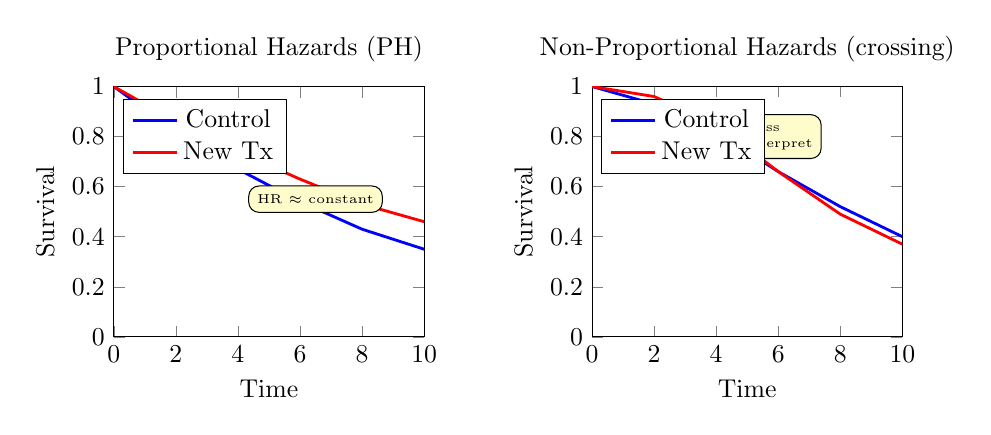
\begin{tikzpicture}[scale=0.93]
  % Left: PH
  \begin{axis}[
    name=PH, width=0.48\linewidth, height=5cm,
    xlabel={Time}, ylabel={Survival}, ymin=0, ymax=1,
    xmin=0, xmax=10, title={Proportional Hazards (PH)},
    legend style={at={(0.03,0.95)},anchor=north west},
    every axis plot/.append style={line width=1.1pt}
  ]
    \addplot[blue] coordinates {(0,1)(2,0.82)(4,0.67)(6,0.54)(8,0.43)(10,0.35)};
    \addlegendentry{Control}
    \addplot[red] coordinates {(0,1)(2,0.86)(4,0.74)(6,0.63)(8,0.53)(10,0.46)};
    \addlegendentry{New Tx}
    \node[draw, fill=yellow!20, font=\tiny, rounded corners] at (axis cs:6.5,0.55) {HR $\approx$ constant};
  \end{axis}
  % Right: non-PH
  \begin{axis}[
    at={(PH.right of south east)}, xshift=2cm,
    anchor=south west, width=0.48\linewidth,
    height=5cm, xlabel={Time}, ylabel={Survival},
    ymin=0, ymax=1, xmin=0, xmax=10,
    title={Non-Proportional Hazards (crossing)},
    legend style={at={(0.03,0.95)},anchor=north west},
    every axis plot/.append style={line width=1.1pt}
  ]
    \addplot[blue] coordinates {(0,1)(2,0.93)(4,0.82)(6,0.66)(8,0.52)(10,0.40)};
    \addlegendentry{Control}
    \addplot[red] coordinates {(0,1)(2,0.96)(4,0.85)(6,0.66)(8,0.49)(10,0.37)};
    \addlegendentry{New Tx}
    \node[draw, fill=yellow!20, font=\tiny, rounded corners, align=center] at (axis cs:4.5,0.80) {Curves cross\\ HR hard to interpret};
  \end{axis}
\end{tikzpicture}

\small Non-PH is no longer exotic—design methods must accommodate it \cite{CrossPharma2020, FDAOS2025}.
\end{frame}

\begin{frame}{HR vs RMST: Understanding the Difference}
\small
\begin{tabular}{@{}p{3cm}p{4.7cm}p{4.7cm}@{}}
\toprule
\textbf{Aspect} & \textbf{Hazard Ratio (HR)} & \textbf{Restricted Mean Survival Time (RMST)}\\
\midrule
Estimand & Instantaneous event rate ratio & \(\mu(L)=\int_0^{L}S(t)dt\) \\
Assumptions & PH — often violated & None — just choose \(L\) wisely \\
Interpretation & Relative; abstract & Absolute — e.g. “X months gained” \\
Non-PH effect & Unstable/misleading & Stable/meaningful \\
Regulatory view & Standard default | RMST supplementary under non-PH \cite{FDAOS2025} \\
\bottomrule
\end{tabular}
\end{frame}

% ====================================================
\section{RMST: Estimand, Interpretation \& Inference}
% ====================================================

\begin{frame}{Defining RMST and Treatment Effect}
\[
\mu(L)=\int_0^L S(t)\,dt,\quad \Delta(L)=\mu_1(L)-\mu_0(L)
\]
\textbf{Interpretation}: average additional event-free time (in normal units) over time horizon \(L\).\\
\textbf{Selecting \(L\)}: must be clinically meaningful and pre-specified in your analysis plan.
\end{frame}

\begin{frame}{Estimating RMST: Methods Overview}
\begin{itemize}
  \item \textbf{Nonparametric}: area under KM curve, with variance via Greenwood or influence functions.
  \item \textbf{Regression-based}:
    \begin{itemize}
      \item IPCW linear regression \cite{Tian2014}.
      \item Pseudo-observations + GAM/GLM \cite{Andersen09, Goetghebeur2013}.
      \item Dependent-censoring models for \(G(t|Z)\) \cite{Wang2018}.
    \end{itemize}
  \item \textbf{Dynamic RMST}: illustrate how \(\Delta(L)\) evolves across different times \cite{DynamicRMST2020}.
\end{itemize}
\end{frame}

% ====================================================
\section{Design: Power \& Sample Size with RMST}
% ====================================================

\begin{frame}{Motivation for RMST-based Design}
\begin{itemize}
  \item Directly targets what will be reported (RMST difference).
  \item Robust to delayed effects/crossover hazards.
  \item Enhances patient understanding (“X months gained”).
\end{itemize}
\end{frame}

\begin{frame}{Analytical vs Bootstrap Engines}
\begin{columns}
\begin{column}{0.5\textwidth}
\textbf{Analytical (fast)}\\
\[
\text{Power}\approx \Phi\left(\frac{|\beta_{\text{eff}}|}{\sigma_N}-z_{1-\alpha/2}\right)
\]
Ideal for sweeping through design scenarios quickly.
\end{column}
\begin{column}{0.5\textwidth}
\textbf{Bootstrap (robust)}\\
\[
\text{Power} = \frac{\#\{p < \alpha\}}{n_{\text{sim}}}
\]
Good when assumptions are unclear; simulates tail behavior.
\end{column}
\end{columns}
\end{frame}

\begin{frame}{Illustrative Power Curves (Synthetic)}
\centering
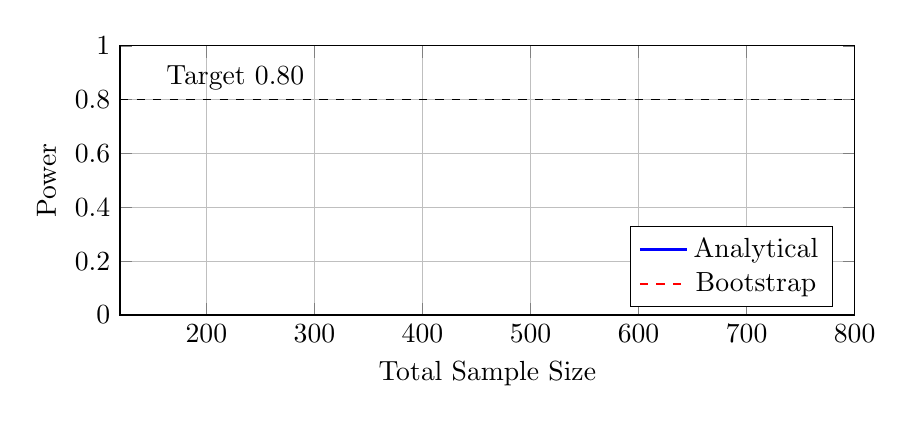
\begin{tikzpicture}
\begin{axis}[
  width=0.9\linewidth, height=5cm,
  xlabel={Total Sample Size}, ylabel={Power},
  ymin=0, ymax=1, xmin=120, xmax=800, grid=both,
  legend pos=south east
]
  \addplot[blue, thick]    {1 - exp(-0.000028*(x-120))}; \addlegendentry{Analytical}
  \addplot[red, thick,dashed] {1 - exp(-0.000023*(x-120))}; \addlegendentry{Bootstrap}
  \draw[dashed] (axis cs:120,0.8)--(axis cs:800,0.8) node[pos=0.05,anchor=south west]{Target 0.80};
\end{axis}
\end{tikzpicture}

\scriptsize Replace with real pilot data results from RMSTSS.
\end{frame}

% ====================================================
\section{The RMSTSS Software}
% ====================================================

\begin{frame}{What Is RMSTSS?}
\begin{itemize}
  \item \textbf{R backend}: implements IPCW, stratified, GAM, dependent-censoring, dynamic RMST models.
  \item \textbf{Shiny frontend}: intuitive interface—upload, map, choose model/goal, visualize, and export.
  \item Two engines: \texttt{analytical} (formula-based) and \texttt{boot} (simulated).
  \item Naming scheme: \texttt{model.goal.method}, e.g., \texttt{MS.ss.boot()} for multiplicative stratified sample-size via bootstrap.
\end{itemize}
\end{frame}

% ---------- Integrated Your Original Content: Screenshot Slide ----------
\begin{frame}{The \texttt{RMSTSS} Shiny App (Original Slide)}
\begin{figure}
  % Replace 'images/app-ss.png' with your actual screenshot path
  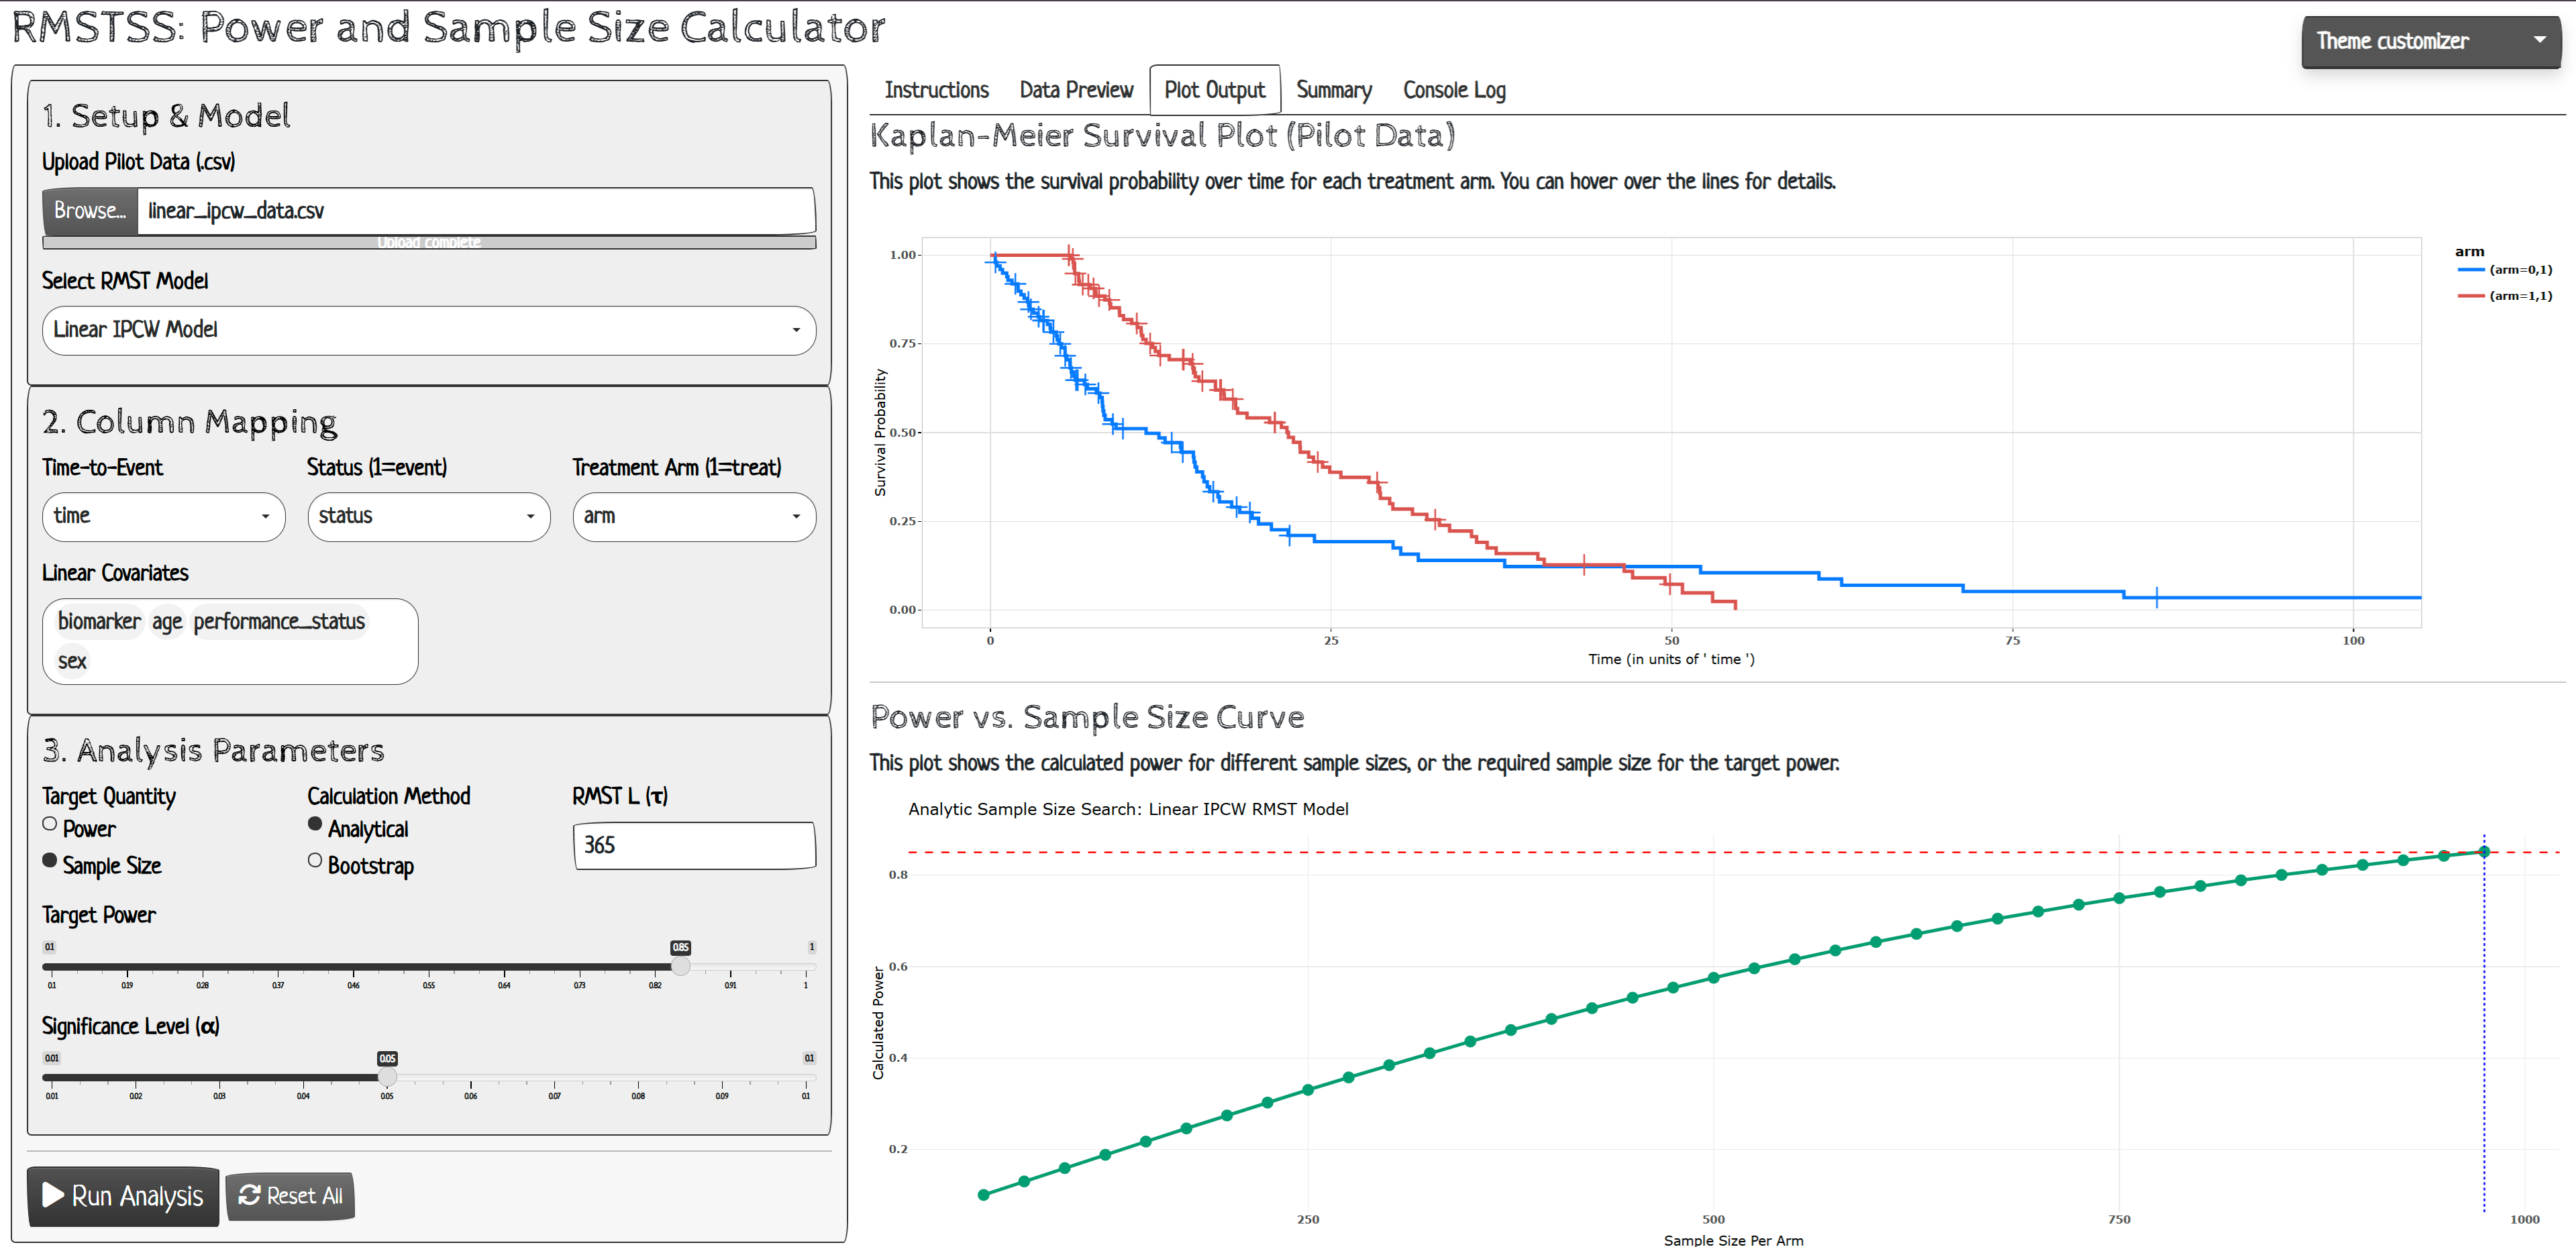
\includegraphics[width=0.9\textwidth]{images/app-ss.png}
  \caption{Shiny application interface showing model selection and result visualization.}
\end{figure}
\end{frame}

% ---------- Integrated Your Original Content: R Example Slide ----------
\begin{frame}[fragile]{Usage Example in R (\texttt{additive.ss.analytical})}
\begin{verbatim}
# Load and prepare data
library(survival)
library(RMSTSS)
colon_death <- colon[colon$etype == 2, ] %>% 
  na.omit()
colon_death$arm    <- ifelse(colon_death$rx == "Obs", 0, 1)
colon_death$strata <- factor(colon_death$extent)

# Calculate sample size
ss_results <- additive.ss.analytical(
  pilot_data   = colon_death,
  time_var     = "time", status_var = "status",
  arm_var      = "arm",  strata_var="strata",
  target_power = 0.80, L = 1825
)
print(ss_results$results_data)
\end{verbatim}
\end{frame}

% ====================================================
\section{Regulatory Guidance \& Reporting}
% ====================================================

\begin{frame}{Regulatory & Reporting Context}
\begin{itemize}
  \item **FDA (2025 Overall Survival Guidance)**: mandates supplementary analysis using RMST when non-PH is anticipated \cite{FDAOS2025}.
  \item **CONSORT 2025**: emphasizes clear, absolute effects; encourages listing RMST alongside HR and medians \cite{CONSORT2025,CONSORT2025BMJ}.
  \item **Cross-Pharma Working Group**: recommends RMST as robust primary/sensitivity estimand in design planning \cite{CrossPharma2020}.
\end{itemize}
\end{frame}

% ====================================================
\section{Best Practices \& Limitations}
% ====================================================

\begin{frame}{Best Practices for RMST Design and Reporting}
\begin{itemize}
  \item Pre-specify \(L\) based on clinical relevance; include a sensitivity range via dynamic RMST.
  \item Adjust for prognostic factors using IPCW or pseudo-observations.
  \item Use dependent-censoring models if informative dropout is plausible.
  \item Report \(\Delta(L)\) with CI, and plot its progression across \(L\).
  \item RMST complements—not necessarily replaces—traditional analyses.
\end{itemize}
\end{frame}

% ====================================================
\section{Conclusion}
% ====================================================

\begin{frame}{Key Take-aways}
\begin{itemize}
  \item RMST: robust, patient-interpretable endpoint, especially valuable under non-PH.
  \item \texttt{RMSTSS}: a comprehensive tool for designing trials using multiple RMST-based models.
  \item Regulatory alignment: increasingly encouraged in design and reporting frameworks.
\end{itemize}
\end{frame}

\begin{frame}{Acknowledgments \& Access}
\textbf{Get the tools:}
\begin{itemize}
  \item Live web app: \texttt{arnab96.shinyapps.io/uthsc-app/}
  \item R package: \texttt{github.com/arnab-aich/RMSTSS}
\end{itemize}
\vspace{0.5em}
\textbf{Acknowledgments:} NSF grant \#2220726, UTHSC BERD support.
\end{frame}

% ====================================================
\appendix
\section{References}
% ====================================================

\begin{frame}[allowframebreaks]{References}
\small
\begin{thebibliography}{99}
\bibitem{RoystonParmar2013}
Royston P, Parmar MKB. Restricted mean survival time: an alternative to the hazard ratio... \emph{Stat Med} 2013;32(20):3377–3388.

\bibitem{Uno2014}
Uno H, Claggett B, Tian L, et al. Moving beyond the hazard ratio... \emph{J Clin Oncol} 2014;32(22):2380–2385.

\bibitem{Tian2014}
Tian L, Zhao L, Wei LJ. Predicting the restricted mean event time with baseline covariates... \emph{Biostatistics} 2014;15(2):222–233.

\bibitem{Andersen09}
Andersen PK, et al. Pseudo-observations in survival analysis... \emph{Stat Methods Med Res} 2010;19:71–99.

\bibitem{Goetghebeur2013}
Andersen PK, Perme MP. Pseudo-values for right-censored data... \emph{Lifetime Data Anal} 2010;16:443–463.

\bibitem{Wang2018}
Wang X, et al. Modeling restricted mean survival time under general censoring... \emph{Lifetime Data Anal} 2018;24(1):54–78.

\bibitem{DynamicRMST2020}
Horiguchi M, Uno H. Dynamic RMST curves for survival analysis... \emph{Contemp Clin Trials Commun} 2020.

\bibitem{QuickGuide2022}
Pak K, Uno H, et al. Restricted Mean Survival Time... \emph{Korean J Radiol} 2022;23(5):760–772.

\bibitem{CrossPharma2020}
Roychoudhury S, et al. Robust design with non-PH: cross-pharma straw-man guidance. 2020 (arXiv).

\bibitem{PHViolations2024}
Miyazawa et al. Proportional Hazards Violations in Phase 3 Cancer Clinical Trials. \emph{J Natl Cancer Inst} 2024.

\bibitem{FDAOS2025}
U.S. FDA. Approaches to Assessment of Overall Survival in Oncology Clinical Trials. Guidance for Industry, 2025.

\bibitem{CONSORT2025}
CONSORT 2025 Statement. EQUATOR Network, 2025.

\bibitem{CONSORT2025BMJ}
CONSORT 2025 Explanation and Elaboration. \emph{BMJ}, 2025.
\end{thebibliography}
\end{frame}

\end{document}
